\documentclass{exam}

\usepackage{units} 
\usepackage{graphicx}
\usepackage[fleqn]{amsmath}
\usepackage{cancel}
\usepackage{float}
\usepackage{mdwlist}
\usepackage{booktabs}
\usepackage{cancel}
\usepackage{polynom}
\usepackage{caption}
\usepackage{fullpage}
\usepackage{comment}
\usepackage{enumerate}
\usepackage{xfrac}

\newcommand{\degree}{\ensuremath{^\circ}} 
\everymath{\displaystyle}

% \begin{figure}[H]
%   \centering
%   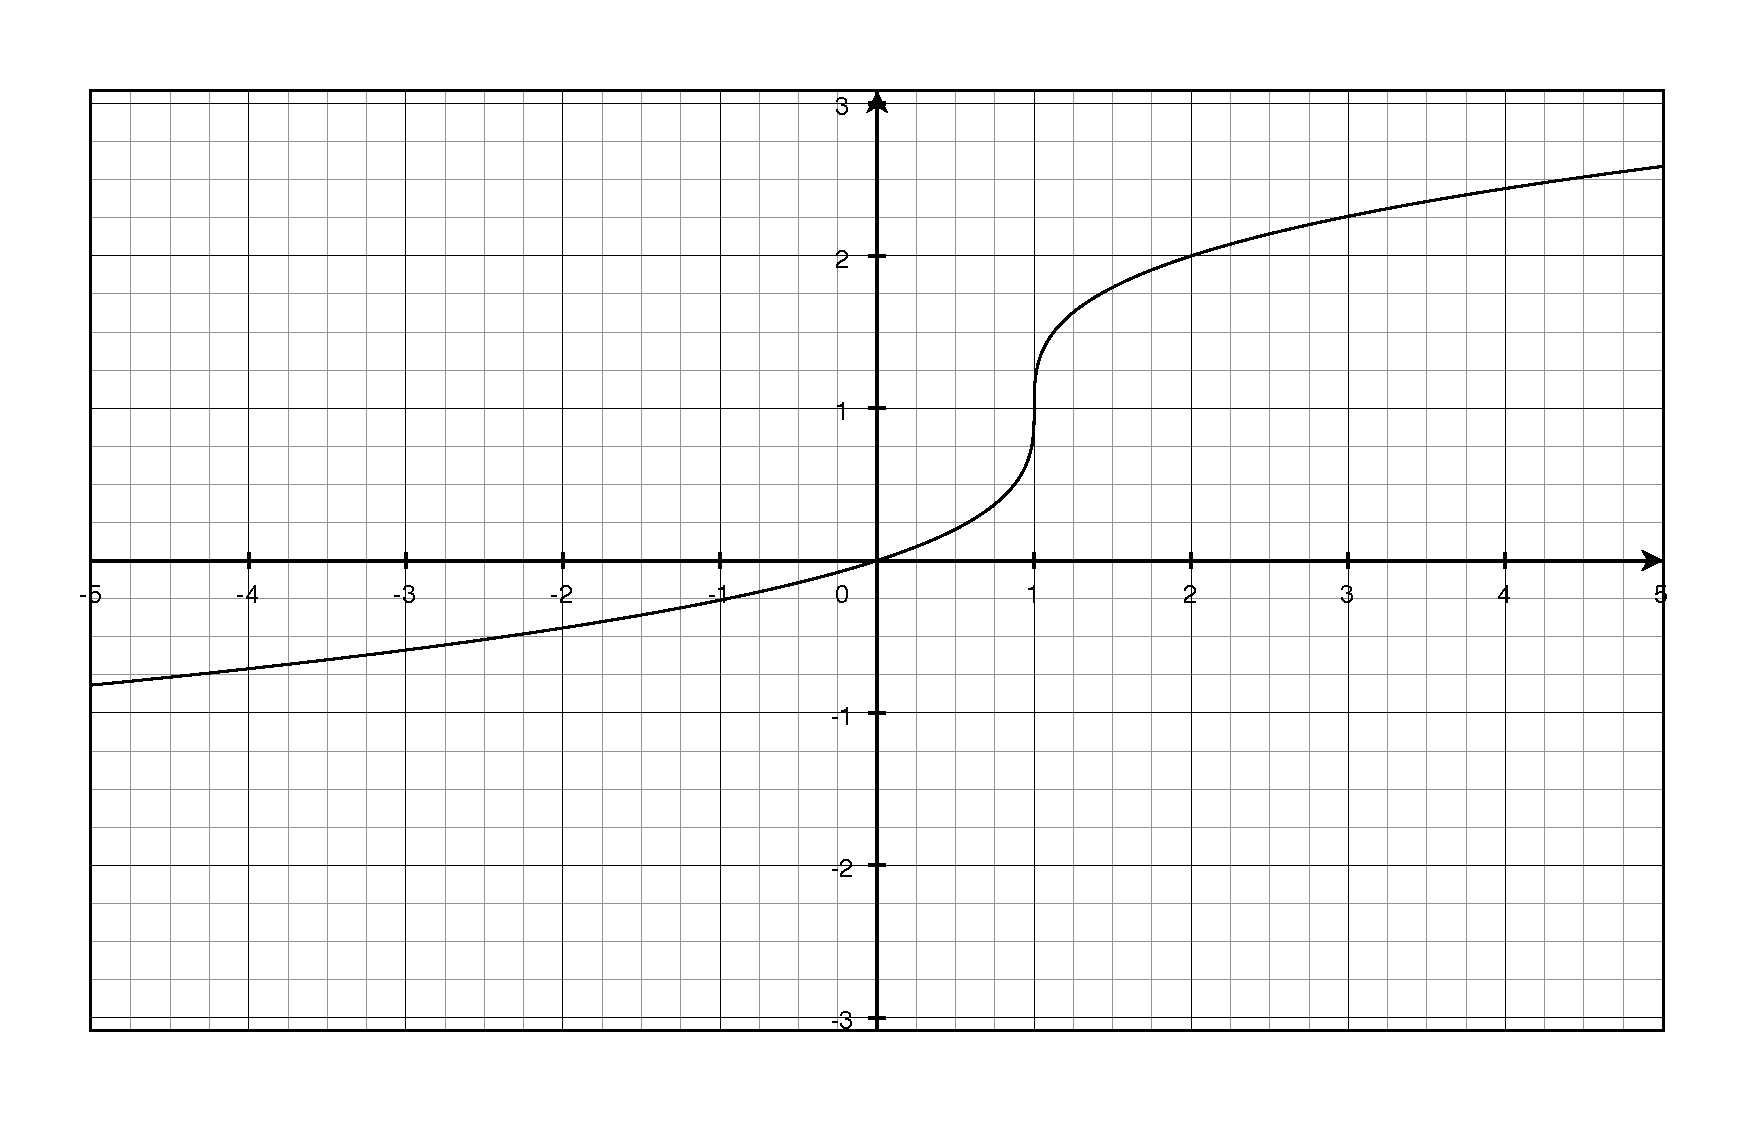
\includegraphics[scale=.3]{question7.eps}
%   \caption*{question 7}
% \end{figure}

% \begin{tabular}{cc}
%   \toprule
%   period & amplitude \\
%     $\pi$ & $2$ \\
%   \bottomrule
% \end{tabular}

\printanswers
\excludecomment{comment}

\ifprintanswers 
  \usepackage{2in1, lscape} 
\fi

\author{}
\date{\today}
\title{Math 142 \\ Homework Five}

\begin{document}

  \maketitle

  \section{Homework}
  Section 5.5: 

  \section{Extra Credit}
  TO DO

  \ifprintanswers

    \pagebreak

    \section{Section 5.5}
    \begin{description}
      \item[9] $f(t) = 10 \sin \left( \frac{2 \pi}{3} t \right)$

      \item[10] $f(t) = 20 \sin \left( \pi t \right)$

      \item[11] $f(t) = 6 \sin \left( 10 t \right)$

      \item[12] $f(t) = 1.2 \sin \left( \frac{\pi}{2} t \right)$
        
      \item[13] $f(t) = 60 \cos \left( 4 \pi t \right)$

      \item[14] $f(t) = 35 \cos \left( \frac{\pi}{4} t \right)$

    \end{description}

  \else
    \vspace{1 cm}
    \begin{quote}
      \begin{em}
        TO DO
      \end{em}
    \end{quote}
    \hspace{1 cm} --Shunryu Suzuki
  \fi

\end{document}

